\documentclass[13pt]{article}
\usepackage[utf8]{inputenc}

\usepackage{polski}
\usepackage{pgfplots}
\usepackage{booktabs} 
\usepackage{fancyhdr}
\pagestyle{fancy}

\begin{document}
 
\begin{titlepage}
\begin{center}

\includegraphics[scale=1.0]{./Pwr_logo/logo_PWr_2.png}
\\
\vspace{1.5cm}
{\Huge Marcin Karasiewicz}\\
\vspace{0.5cm}
{\Huge Rafał Kowalski}
\\
\begin{Large}
\vspace{1.0cm}
Projektowanie algorytmów \\ i metody sztucznej inteligencji \\
\vspace{1.0cm}
Grafy - "Jak dojadę?"
\end{Large}
\end{center}
\newpage
\tableofcontents 
\end{titlepage}
\newpage

\section{Założenia projektowe}

Projekt zakłada stworzenie programu, który wyszukuje najbardziej optymalną czasowo trasę między zadanymi stacjami tramwajowymi we Wrocławiu. Aby to osiągnąć program ma wykorzystywać 3 algorytmy grafowe: Breath First Search, Deep First Search oraz A Star. W projekcie można wyróżnić następujące zadania:
\begin{itemize}
\item Pobranie danych dotyczących połączeń tramwajowych ze strony miasta 
\item Przeparsowanie nadmiaru danych z plików w formacie *.xml na potrzebne dla programu dane w formacie *.csv
\item Implementacja tworzenia grafu na podstawie danych z plików *.csv
\item Wizualizacja grafu w programie Gnuplot
\item Implementacja zadanych algorytmów grafowych
\item Wizualizacja działania algorytmów animacją w programie Gnuplot
\item Analiza działania algorytmów 
\item Stworzenie graficznego interfejsu użytkownika
\item Wyciagnięcie wniosków
\end{itemize}

\section{Parser danych XML }

Parser danych został napisany w Pythonie w wersji 3.
Użyto biblioteki Etree, służącej do poruszania się po plikach XML.
Parser wyszukuje korzeń, następnie szuka \textit{wariantu} trasy, następnie wyszukuje na danym \textit{wariancie} wszystkie \textit{przystanki}, a następnie odczytuje z nich ich \textit{id},
\textit{nazwę}, \textit{ulicę} oraz \textit{czas}, ile potrzebuję tramwaj na dojechanie do kolejnej stacji na trasie.
Na końcu dane te zostają zapisane do pliku \textit{*.cvs}

\section{Implementacja tworzenia grafu} 

Przeparsowane dane zostały podzielone na pliki zawierające pojedyńcze trasy tramwajowe. Graf jest tworzony dynamicznie podczas odczytu danych z tych plików. Algorytm tworzenia grafu prezentuje się następująco:
\begin{enumerate}
\item{Otwórz plik z trasą tramwajową.}
\item{Wczytaj nazwę tramwaju.}
\item{Wczytaj dane o pierwszej stacji na trasie z kolejnej linii pliku.}
\item{Przeszukaj graf w celu sprawdzenia, czy istnieje w grafie już stacja o takich parametrach, jak właśnie wczytane.}
\item{Jeśli istnieje: ustaw na nią wskaźnik \textit{acctual}; jeśli nie istnieje: utwórz w grafie nową stację o parametrach takich, jak wczytane dane i ustaw na nią wskaźnik \textit{acctual}.}
\item{Wczytaj dane o kolejnej stacji na trasie z kolejnej linii pliku.}
\item{Przeszukaj graf w celu sprawdzenia, czy istnieje w grafie już stacja o takich parametrach, jak właśnie wczytane.}
\item{Jeśli istnieje: ustaw na nią wskaźnik \textit{next}; jeśli nie istnieje: utwórz w grafie nową stację o parametrach takich, jak wczytane dane i ustaw na nią wskaźnik \textit{next}.}
\item{Utwórz połączenie do sąsiada stacji, na którą wskazuje \textit{acctual} o poarametrach: Sąsiadująca stacja - stacja, na którą wskazuje \textit{next}; Czas podróży do sąsiada - wczytany czas; Nazwa tramwaju realizującego połączenie - wczytana nazwa z początku pliku.}
\item{Ustaw wskaźnik \textit{acctual} na stację, na którą wskazuje \textit{next}.}
\item{Powatarzaj kroki od 6. do10. aż do końca danych w pliku.}
\end{enumerate}
Algorytm Wykonywany jest dla wszystkich plików zawierających dane o połączeniach tramwajowych.\\
Kluczowym elementem algorytmu jest krok 10. Zapewnia on tworzenie zawsze odpowiednich połączeń do sąsiadów kolejno wczytywanych stacji.

%%%%%%%%%%%%%%%%%%%%%%%%%%%%%%%%%%%%%%%%%%%%%%%%

\section{Breadth First Search}

\subsection{Opis}
Algorytm, jak jego nazwa wskazuje, szuka trasy między zadanymi stacjami przeszukując graf wszerz. Zapewnia to znalezienie zawsze najlepszej trasy, ale kosztem zbadania dużej ilości połączeń. Wyszukana przez algorytm trasa stanowi wzorzec do porównania dla tras znalezionych przez pozostałe algorytmy.

\newpage
\subsection{Implementacja}

Realizację algorytmu zapewnia kolejka na którą odkładamy, najpierw stację początkową. Kolejne kroki powtarzają się do znalezienia stacji końcowej, lub opustoszenia kolejki: 
\begin{enumerate}
\item Zdejmij stację z kolejki.
\item Sprawdź, czy zdjęta staja nie jest stacją końcową (jeśli jest, to następny krok nie jest już wykonywany).
\item Dodaj do kolejki wszystkich jej sąsiadów, którzy nie zostali wcześniej dodani.
\end{enumerate}
Sprawdzenie, czy stacja została już odwiedzona zapewnia kolorowanie stacji numerami 0 - stacja nie odwiedzona, 1 - stacja znajduje się już w kolejce, 3 - wszyscy sąsiedzi tej stacji zostali już dodani do kolejki. \\
Gdy algorytm znajdzie stację końcową odkłada ją na stos, następnie kolejno stacje, z których do niej dojechał, aż do stacji początkowej. Pozwala to na późniejsze wypisanie trasy ze stosu oraz lokalizacji stacji na trasie, potrzebnych do wizualizacji.


\subsection{Testy}
\begin{tabular}{|c|c|c|c|} \hline
Trasa & Czas przejazdu  & Zbadane połączenia & Czas algorytmu [ms]\\
\hline \hline
 LEŚNICA - GAJ & 51 & 173 & $1.5007e-04$ \\
 \hline
 KOZANÓW - BISKUPIN & 38 & 175 &  $1.6949e-04$ \\
 \hline
 RYNEK - BISKUPIN & 20 & 162 & $1.6641e-04$ \\
 \hline
 PL.GRUNWALDZKI - DW GŁÓWNY & 9 & 32 &  $4.2369e-05$\\
 \hline
\end{tabular}

\newpage
\begin{itemize}
\item Długa trasa między stacjami bardzo odległymi na krańcach grafu
\end{itemize}
\hspace{1.5cm} Stacje: LEŚNICA - GAJ \\\\
Id: 21030   - 18201\\
Czas przejazdu: 51\\
Liczba zbadanych połączeń: 173\\
Czas działania algorytmu: 0.000150065 ms
\begin{figure}[hp]
\centering
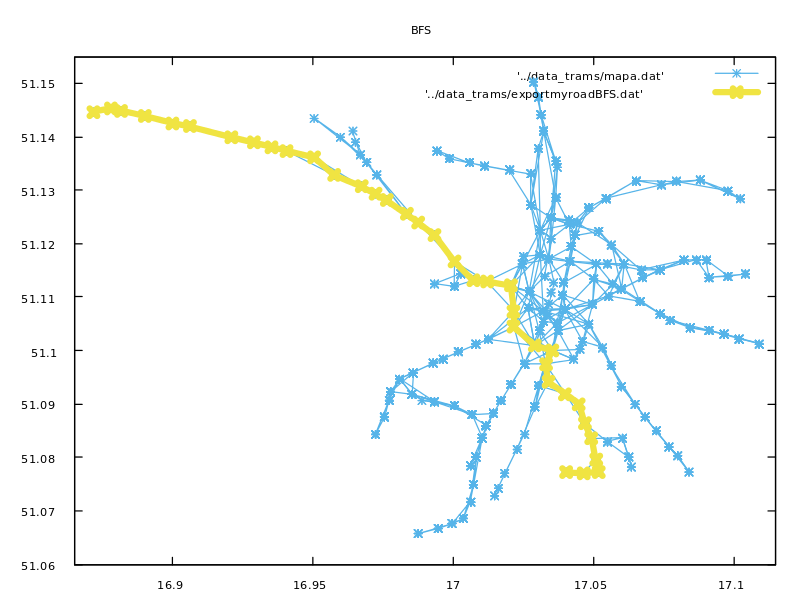
\includegraphics[width=1\textwidth]{wykresy/LES_GAJ_BFS.png}
\caption{Leśnica - Gaj BFS}
\end{figure}

Czy zaleziona trasa jest optymalna?\\
Trasa wzorcowa

\newpage
\begin{itemize}
\item Trasa między stacjami krańcowymi grafu
\end{itemize}
\hspace{1.5cm}Stacje: KOZANÓW - BISKUPIN\\\\
Id: 12610   - 24416\\
Czas przejazdu: 38\\
Liczba zbadanych połączeń: 175\\
Czas działania algorytmu: 0.000169492 ms\\
\begin{figure}[hp]
\centering
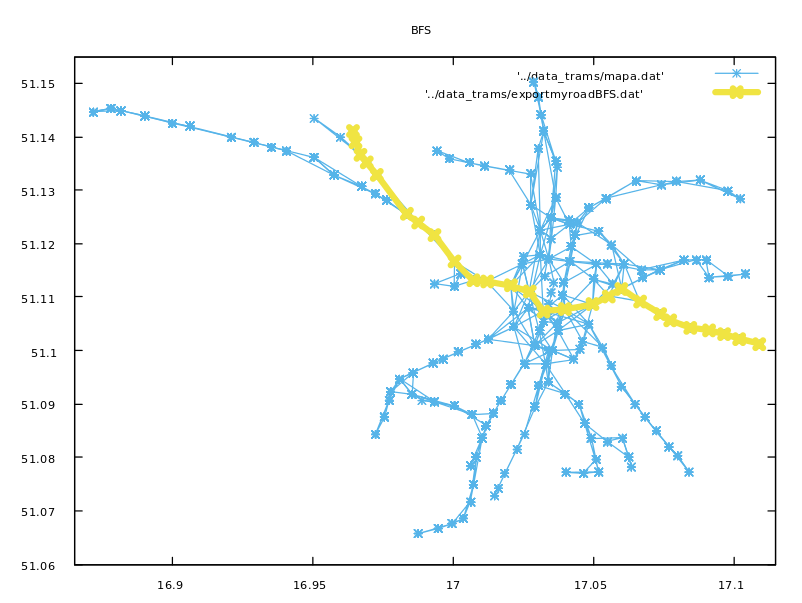
\includegraphics[width=1\textwidth]{wykresy/KOZA_BIS_BFS.png}
\caption{Kozanów - Biskupin BFS}
\end{figure}

Czy zaleziona trasa jest optymalna?\\
Trasa wzorcowa

\newpage
\begin{itemize}
\item Trasa między stacją z środka do stacji na krańcu grafu
\end{itemize}
\hspace{1.5cm} Stacje: RYNEK - BISKUPIN\\\\
Id: 10003 - 24416\\
Czas przejazdu: 20\\
Liczba zbadanych połączeń: 162\\
Czas działania algorytmu: 0.000166407 ms\\
\begin{figure}[hp]
\centering
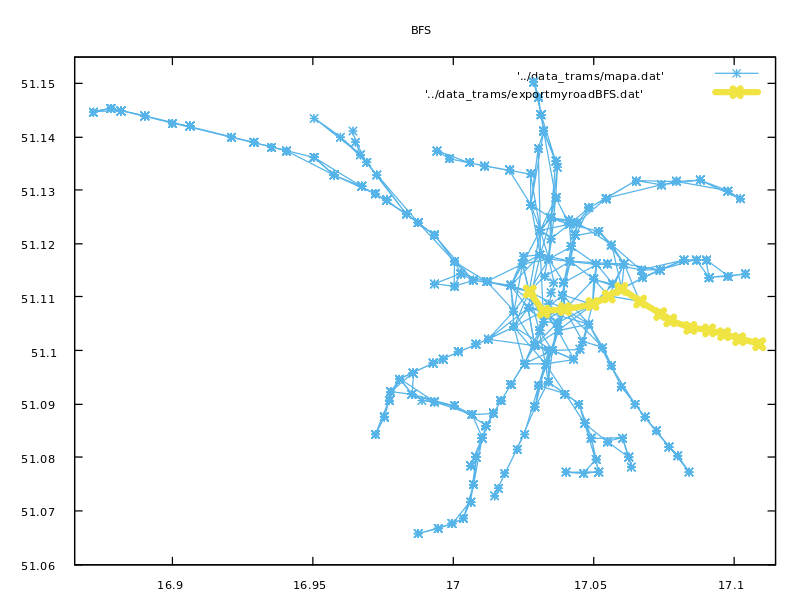
\includegraphics[width=1\textwidth]{wykresy/RYN_BIS_BFS.png}
\caption{Rynek - Biskupin BFS}
\end{figure}

Czy zaleziona trasa jest optymalna?\\
Trasa wzorcowa

\newpage
\begin{itemize}
\item Trasa między stacjami znajdującym się w środku grafu
\end{itemize}
\hspace{1.5cm} Stacje: PL.GRUNWALDZKI - DW GŁÓWNY \\\\
Id: 20823  - 10226\\
Czas przejazdu: 9\\
Liczba zbadanych połączeń: 32\\
Czas działania algorytmu: $4.2369e-05$ ms\\
\begin{figure}[hp]
\centering
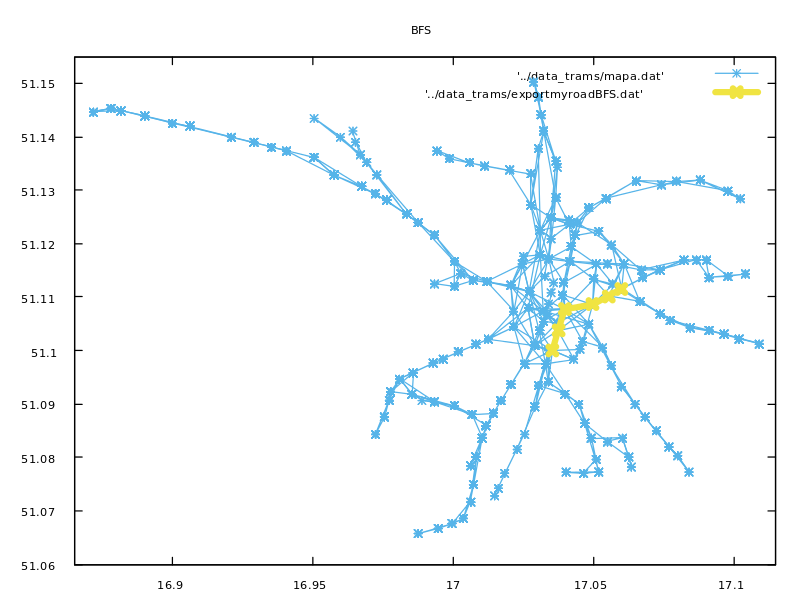
\includegraphics[width=1\textwidth]{wykresy/PLA_GLO_BFS.png}
\caption{PL. Grunwaldzki - Dworzec Gł. BFS}
\end{figure}

Czy zaleziona trasa jest optymalna?\\
Trasa wzorcowa

%%%%%%%%%%%%%%%%%%%%%%%%%%%%%%%%%%%%%%%%%%%%%%%%%%%%
\newpage

\section{Deep First Search}

\subsection{Opis}
Algorytm, jak jego nazwa wskazuje, szuka trasy między zadanymi stacjami przeszukując graf wgłąb. Oznacza to, że w przeciwieństwie do BFS, w  pierwszej kolejności przeszukuje trasę, którą zaczął badać, do jej końca i dopiero potem zaczyna przeszukiwać kolejną trasę. Powoduje to, w większości przypadków, znalezienie dłuższej trasy w porównaniu do trasy wzorcowej wyznaczonej przez BFS, jednakże kosztem mniejszej ilości zbadanych połączeń. 

\subsection{Implementacja}
Różnica w implementacji algorytmu DFS względem BFS sprowadza się do zamienienia kolejki na stos.


\subsection{Testy}
\begin{tabular}{|c|c|c|c|} \hline
Trasa & Czas przejazdu  & Zbadane połączenia & Czas algorytmu [ms]\\
\hline \hline
 LEŚNICA - GAJ & 51 & 45 &  $3.0945e-05$ \\
 \hline
 KOZANÓW - BISKUPIN & 48 & 146 &  $1.1721e-04$ \\
 \hline
 RYNEK - BISKUPIN & 30 & 138 & $8.4303e-05$ \\
 \hline
 PL.GRUNWALDZKI - DW GŁÓWNY & 24 & 96 &   $1.0685e-04$\\
 \hline
\end{tabular}

\newpage

\begin{itemize}
\item Długa trasa między stacjami bardzo odległymi na krańcach grafu
\end{itemize}
\hspace{1.5cm} Stacje: LEŚNICA - GAJ \\\\
Id: 21030   - 18201\\
Czas przejazdu: 51\\
Liczba zbadanych połączeń: 45\\
Czas działania algorytmu: $3.0945e-05$ ms
\begin{figure}[hp]
\centering
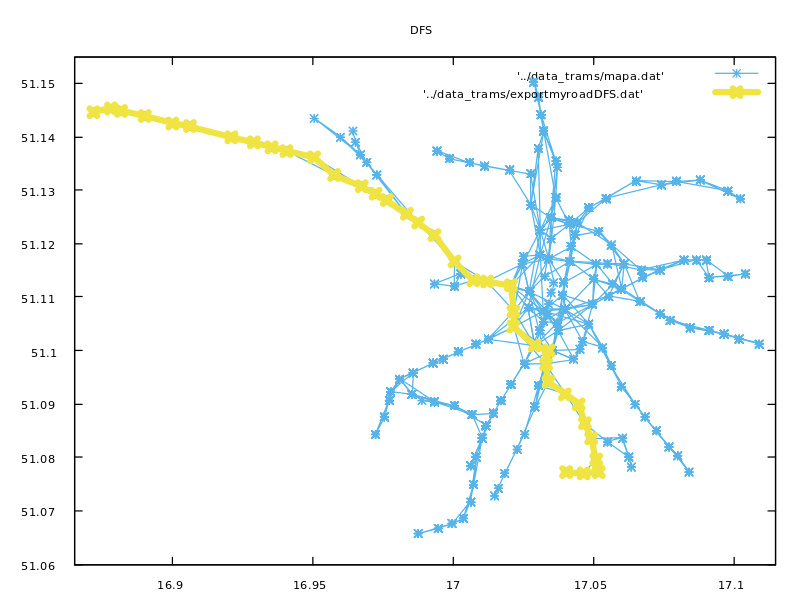
\includegraphics[width=1\textwidth]{wykresy/LES_GAJ_DFS.png}
\caption{Leśnica - Gaj DFS}
\end{figure}

Czy zaleziona trasa jest optymalna?\\
Trasa taka sama jak przy BFS. Wynika to z przypadkowego ustawienia danych w grafie i szybkiego przeszukania szukanej trasy, przez co liczba zbadanych połączeń jest kilkukrotnie mniejsza niż w BFS.

\newpage
\begin{itemize}
\item Trasa między stacjami krańcowymi grafu
\end{itemize}
\hspace{1.5cm}Stacje: KOZANÓW - BISKUPIN\\\\
Id: 12610   - 24416\\
Czas przejazdu: 48\\
Liczba zbadanych połączeń: 146\\
Czas działania algorytmu: 0.000117204 ms\\
\begin{figure}[hp]
\centering
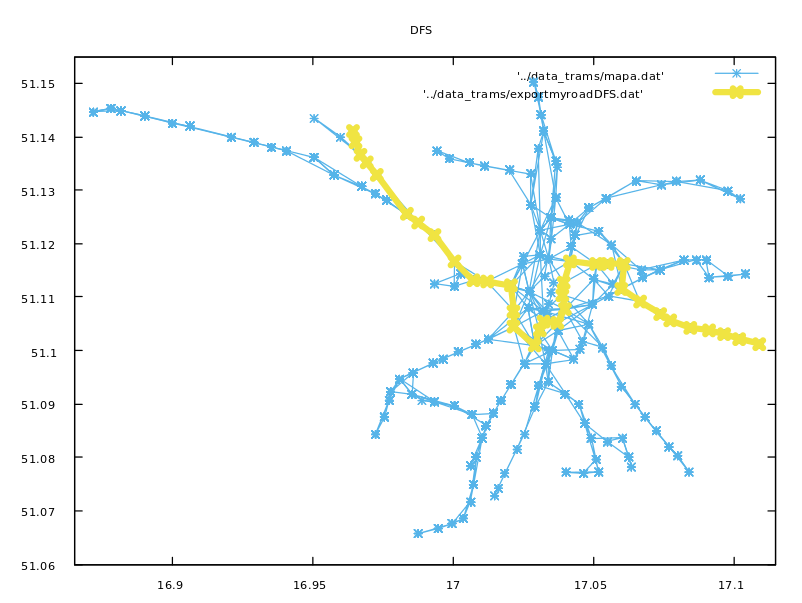
\includegraphics[width=1\textwidth]{wykresy/KOZA_BIS_DFS.png}
\caption{Kozanów - Biskupin DFS}
\end{figure}

Czy zaleziona trasa jest optymalna?\\
Trasa o 10 minut dłuższa niż trasa znaleziona przez BFS. Różnica 10 minut nie dyskwalifikuje tej trasy z bycia optymalną. Można ją polecić osobą chcącym zwiedzić miasto zza szyby tramwaju. Algorytmowi wystarzczyło o 29 mniej zbadanych połączeń niż przy BFS, by wyznaczyć trasę.

\newpage
\begin{itemize}
\item Trasa między stacją z środka do stacji na krańcu grafu
\end{itemize}
\hspace{1.5cm} Stacje: RYNEK - BISKUPIN\\\\
Id: 10003 - 24416\\
Czas przejazdu: 30\\
Liczba zbadanych połączeń: 138\\
Czas działania algorytmu: $8.4303e-05$ ms\\
\begin{figure}[hp]
\centering
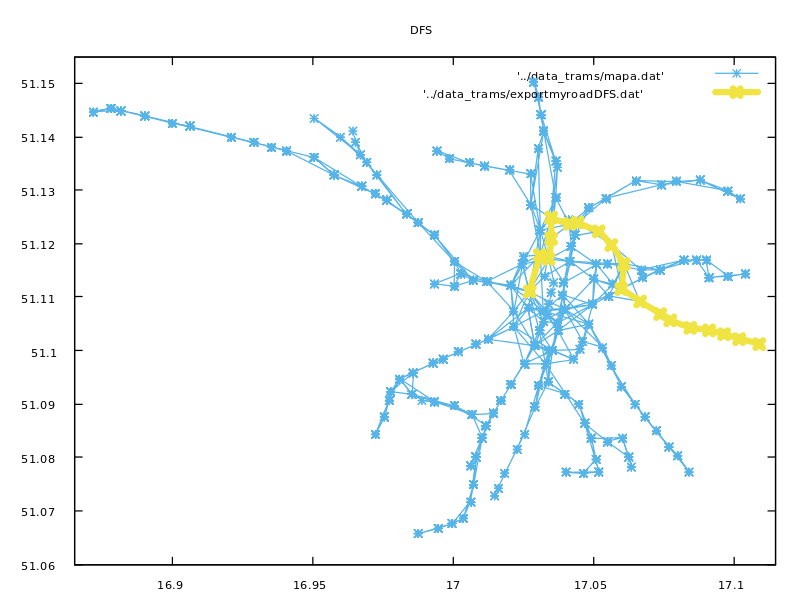
\includegraphics[width=1\textwidth]{wykresy/RYN_BIS_DFS.png}
\caption{Rynek - Biskupin DFS}
\end{figure}

Czy zaleziona trasa jest optymalna?\\
Trasa o 10 minut dłuższa niż trasa znaleziona przez BFS. Różnica 10 minut nie dyskwalifikuje tej trasy z bycia optymalną. Algorytmowi wystarzczyło o 24 mniej zbadanych połączeń niż przy BFS, by wyznaczyć trasę.

\newpage
\begin{itemize}
\item Trasa między stacjami znajdującym się w środku grafu
\end{itemize}
\hspace{1.5cm} Stacje: PL.GRUNWALDZKI - DW GŁÓWNY \\\\
Id: 20823  - 10226\\
Czas przejazdu: 24\\
Liczba zbadanych połączeń: 96\\
Czas działania algorytmu: 0.00010685 ms\\
\begin{figure}[hp]
\centering
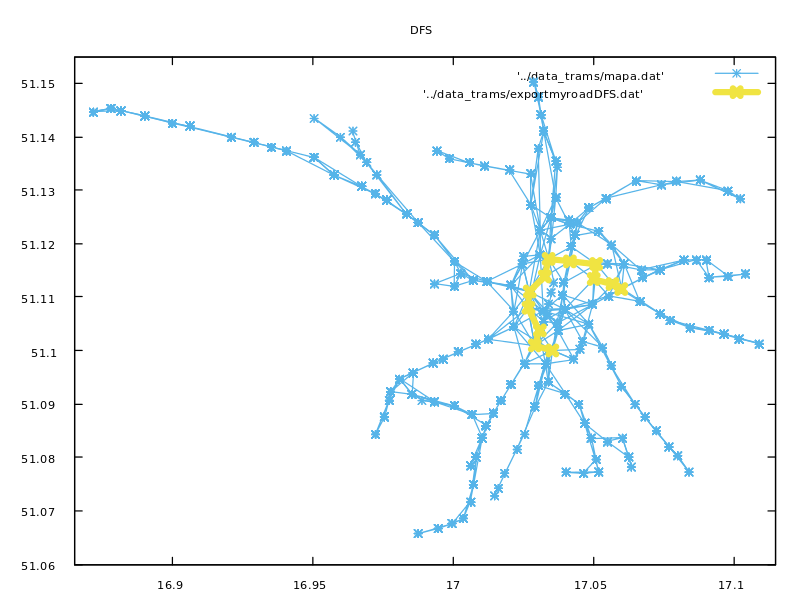
\includegraphics[width=1\textwidth]{wykresy/PLA_GLO_DFS.png}
\caption{PL. Grunwaldzki - Dworzec Gł. DFS}
\end{figure}

Czy zaleziona trasa jest optymalna?\\
Trasa o 15 minut dłuższa niż trasa znaleziona przez BFS. Różnica 15 minut dyskwalifikuje tą trasę z bycia optymalną. Podróżnik najprawdopodobniej ceni sobie najszybszy przejazd między stacjami w mieście, będącymi stosunkowo blisko siebie. Algorytm potrzebował o 64 więcej zbadanych połączeń niż BFS. Wynika to z badania wgłąb tras nie prowadzących do celu przed zbadaniem szukanej trasy.

%%%%%%%%%%%%%%%%%%%%%%%%%%%%%%%%%%%%%%%%%%%%%%%%%%%%%%%%%%

\section{A Star}

\subsection{Opis}
Algorytm by wybrać połączenie, które w danym kroku będzie badać korzysta z funkcji:\\
$f=g+300*h$, gdzie:\\\\
$g$ - suma odległości między stacjami na trasie od stacji początkowej do stacji, na której właśnie jest algorytm,\\\\
$h$ - heurystyka, będąca odległością w linii prostej między stacją, na której właśnie jest algorytm, a stacją końcową.\\\\
Waga $h$ musiała zostać zwielokrotniona w stosunku do wagi $g$, ponieważ zrealizowany graf jest mapą miasta ze współrzędnymi geograficznymi, gdzie przy tak małych wartościach $g$ i $h$, $h$ traciła zupełnie na swojej wartości.
Funkcja $f$ jest poprawna dla grafów będących mapą, gdzie długość krawędzi odpowiada odległości między wierzchołkami. W naszym przypadku długość krawędzi stanowi czas przejazdu między stacjami, który jest proporcjonalny do odległości. Pozwala to na używanie tej funkcji, jednak dla dokładności algorytmu stosujemy odległość rzeczywistą.\\
Algorytm zawsze bada to połączenie, dla którego funkcja $f$ przyjmuje najmniejszą wartość w porównaniu do pozostałych możliwych do zbadania w danym kroku połączeń.

\subsection{Implementacja}
W przypadku algorytmu A* zamiast kolejki czy stosu wykorzystujemy listę. Wybór ten został podyktowany potrzebą dostępu do jej dowolnego elementu. Procedura algorytmu w stosunku do BFS została wzbogacona o wybór stacji którą wybierzemy do badań trasy i usuniemy z listy. Wybór podyktowany jest warunkiem podanym w opisie algorytmu. Jego realizację zapewnia badanie długości wektora, będącego różnicą wektorów o początku zawsze w punkcie $[0,0]$ i końcach o współrzędnych geograficznych stacji:\\\\
element $g$ - suma długości różnic wektorów sąsiadujących ze sobą stacji na trasie od stacji początkowej, do stacji którą sprawdza algorytm,\\\\
element $h$ - długość różnicy wektorów stacji końcowej i stacji, którą sprawdza algorytm.\\\\
Algorytm sprawdza w ten sposób wszystkie stacje do których może dojechać ze stacji, na której jest w danej chwili i wybiera przejście do stacji, dla której funkcja $f$ przyjmuje najmniejszą wartość.

\newpage
\subsection{Testy}

\begin{tabular}{|c|c|c|c|} \hline
Trasa & Czas przejazdu  & Zbadane połączenia & Czas algorytmu [ms]\\
\hline \hline
 LEŚNICA - GAJ & 51 & 34 &  $4.2438e-05$ \\
 \hline
 KOZANÓW - BISKUPIN & 38 & 33 &  $5.6273e-05$ \\
 \hline
 RYNEK - BISKUPIN & 20 & 21 & $2.4711e-05$ \\
 \hline
 PL.GRUNWALDZKI - DW GŁÓWNY & 9 & 5 &  $1.0836e-05$\\
 \hline
\end{tabular}

\begin{itemize}
\item Długa trasa między stacjami bardzo odległymi na krańcach grafu
\end{itemize}
\hspace{1.5cm} Stacje: LEŚNICA - GAJ \\\\
Id: 21030   - 18201\\
Czas przejazdu: 51\\
Liczba zbadanych połączeń: 34\\
Czas działania algorytmu: $4.2438e-05$ ms\\
\begin{figure}[hp]
\centering
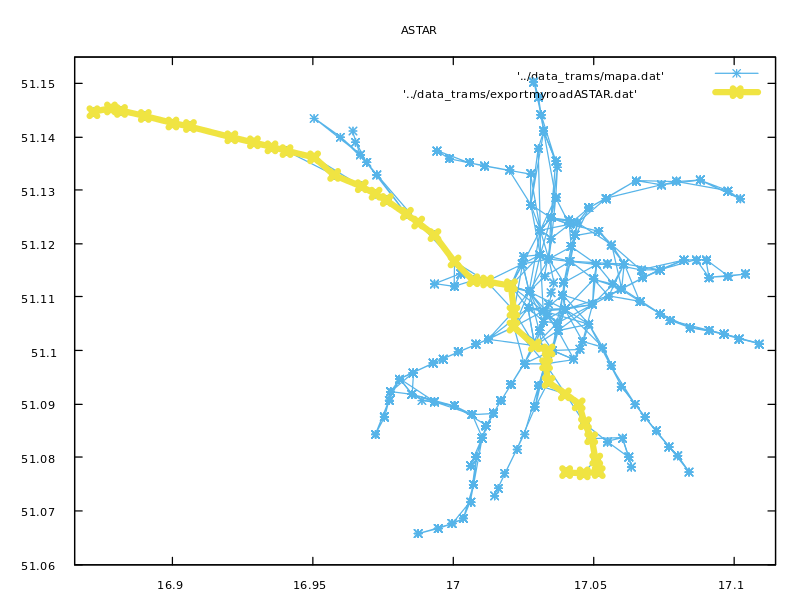
\includegraphics[width=1\textwidth]{wykresy/LES_GAJ_ASTAR.png}
\caption{Leśnica - Gaj ASTAR}
\end{figure}

Czy zaleziona trasa jest optymalna?\\
Trasa taka sama jak przy BFS. Potwierdza to skuteczność algorytmu, który potrzebował wielokrotnie mniej zbabadanych połączeń niż BFS i mniej niż DFS, by wyznaczyć najoptymalniejszą trasę.

\newpage
\begin{itemize}
\item Trasa między stacjami krańcowymi grafu
\end{itemize}
\hspace{1.5cm}Stacje: KOZANÓW - BISKUPIN\\\\
Id: 12610   - 24416\\
Czas przejazdu: 38\\
Liczba zbadanych połączeń: 33\\
Czas działania algorytmu: $5.6273e-05$ ms\\
\begin{figure}[hp]
\centering
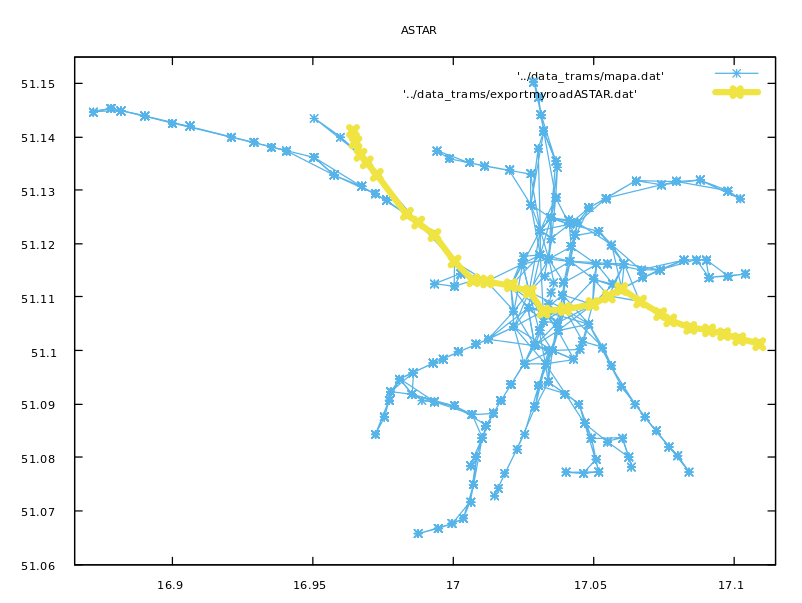
\includegraphics[width=1\textwidth]{wykresy/KOZA_BIS_ASTAR.png}
\caption{Kozanów - Biskupin ASTAR}
\end{figure}

Czy zaleziona trasa jest optymalna?\\
Trasa taka sama jak przy BFS. Potwierdza to skuteczność algorytmu, który potrzebował wielokrotnie mniej zbabadanych połączeń niż BFS i DFS, by wyznaczyć najoptymalniejszą trasę.

\newpage
\begin{itemize}
\item Trasa między stacją z środka do stacji na krańcu grafu
\end{itemize}
\hspace{1.5cm} Stacje: RYNEK - BISKUPIN\\\\
Id: 10003 - 24416\\
Czas przejazdu: 20\\
Liczba zbadanych połączeń: 21\\
Czas działania algorytmu: $2.4711e-05$ ms\\
\begin{figure}[hp]
\centering
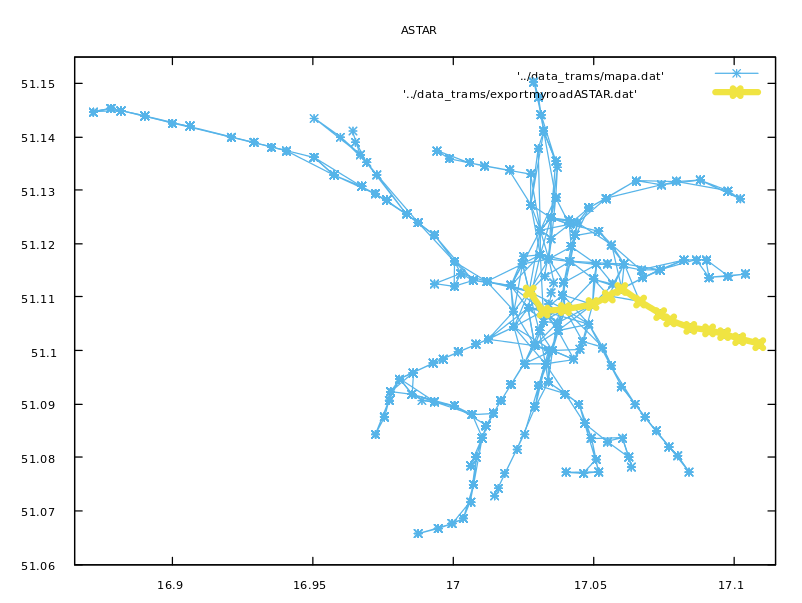
\includegraphics[width=1\textwidth]{wykresy/RYN_BIS_ASTAR.png}
\caption{Rynek - Biskupin ASTAR}
\end{figure}

Czy zaleziona trasa jest optymalna?\\
Trasa taka sama jak przy BFS. Potwierdza to skuteczność algorytmu, który potrzebował wielokrotnie mniej zbabadanych połączeń niż BFS i DFS, by wyznaczyć najoptymalniejszą trasę.

\newpage
\begin{itemize}
\item Trasa między stacjami znajdującym się w środku grafu
\end{itemize}
\hspace{1.5cm} Stacje: PL.GRUNWALDZKI - DW GŁÓWNY \\\\
Id: 20823  - 10226\\
Czas przejazdu: 9\\
Liczba zbadanych połączeń: 5\\
Czas działania algorytmu: $1.0836e-05$ ms\\
\begin{figure}[hp]
\centering
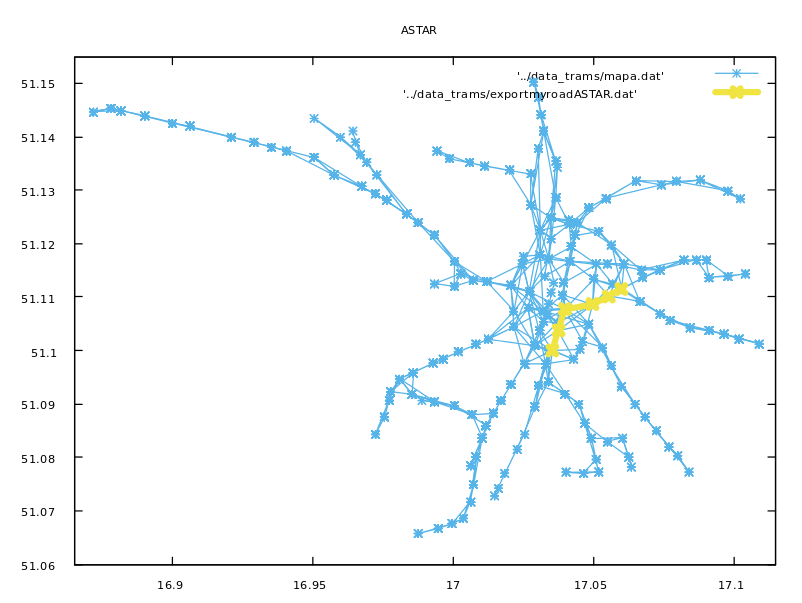
\includegraphics[width=1\textwidth]{wykresy/PLA_GLO_ASTAR.png}
\caption{PL. Grunwaldzki - Dworzec Gł. ASTAR}
\end{figure}

Czy zaleziona trasa jest optymalna?\\
Trasa taka sama jak przy BFS. Potwierdza to skuteczność algorytmu, który potrzebował wielokrotnie mniej zbabadanych połączeń niż BFS i DFS, by wyznaczyć najoptymalniejszą trasę.

%%%%%%%%%%%%%%%%%%%%%%%%%%%%%%%%%%%%%%%%%%%%%
\newpage

\section{Wizualizacja w Gnuplot}
Do wszelkiej wizualizacji został wykorzystany darmowy program Gnuplot. Struktura grafu jest zapisywana przez program do pliku \textit{mapa.dat}. Znajdowane trasy zapisywane są do plików \textit{exportmyroadBFS.dat}, \textit{exportmyroadDFS.dat}, \textit{exportmyroadASTAR.dat}. Zapisane w plikach współrzędne geograficzne stacji są rysowane przez program Gnuplot. Dynamiczna edycja plików zawierających trasy, podczas wykonywania algorytmów szukających, zapewnia animację wyszukiwania trasy i pozwala na obserwację sposobu działania każdego z algorytmów. Należy pamiętać, że przy pomiarach czasu wykonywania algorytmu należy zakomentować części kodu odpowiadające za animację.
%%%%%%%%%%%%%%%%%%%%%%%%%%%%%%%%%%%%%%%%%%%%%%

\section{GUI }

Graficzny interfejs użytkownika został napisany w Pythonie w wersji 3.
Użyto biblioteki Tkinter, służącej do tworzenia aplikacji okienkowych.
Interfejs jest prosty: składa się z dwóch Combobox'ów, z których wybiera się stację początkową i końcową. Kolejnymi elementami są dwa przyciski - pierwszy odpowiedzialny za wyszukanie połącznia oraz drugi odpowiedzialny za poprawne zamknięcie binarki. Dane do binarki przekazywane są za pomocą przechwycenia strumieni wejścia i wyjśćia.

%%%%%%%%%%%%%%%%%%%%%%%%%%%%%%%%%%%%%%%%%%%%
\newpage

\section{Wnioski}

\begin{itemize}
\item Breadth First Search
\end{itemize}
\begin{tabular}{|c|c|c|c|} \hline
Trasa & Czas przejazdu  & Zbadane połączenia & Czas algorytmu [ms]\\
\hline \hline
 LEŚNICA - GAJ & 51 & 173 & $1.5007e-04$ \\
 \hline
 KOZANÓW - BISKUPIN & 38 & 175 &  $1.6949e-04$ \\
 \hline
 RYNEK - BISKUPIN & 20 & 162 & $1.6641e-04$ \\
 \hline
 PL.GRUNWALDZKI - DW GŁÓWNY & 9 & 32 &  $4.2369e-05$\\
 \hline
\end{tabular}

\begin{itemize}
\item Deep First Search
\end{itemize}
\begin{tabular}{|c|c|c|c|} \hline
Trasa & Czas przejazdu  & Zbadane połączenia & Czas algorytmu [ms]\\
\hline \hline
 LEŚNICA - GAJ & 51 & 45 &  $3.0945e-05$ \\
 \hline
 KOZANÓW - BISKUPIN & 48 & 146 &  $1.1721e-04$ \\
 \hline
 RYNEK - BISKUPIN & 30 & 138 & $8.4303e-05$ \\
 \hline
 PL.GRUNWALDZKI - DW GŁÓWNY & 24 & 96 &   $1.0685e-04$\\
 \hline
\end{tabular}

\begin{itemize}
\item A Star
\end{itemize}
\begin{tabular}{|c|c|c|c|} \hline
Trasa & Czas przejazdu  & Zbadane połączenia & Czas algorytmu [ms]\\
\hline \hline
 LEŚNICA - GAJ & 51 & 34 &  $4.2438e-05$ \\
 \hline
 KOZANÓW - BISKUPIN & 38 & 33 &  $5.6273e-05$ \\
 \hline
 RYNEK - BISKUPIN & 20 & 21 & $2.4711e-05$ \\
 \hline
 PL.GRUNWALDZKI - DW GŁÓWNY & 9 & 5 &  $1.0836e-05$\\
 \hline
\end{tabular}\\\\\\
Czasy działania algorytmów BFS i DFS rosną odpowiednio ze wzrostem liczby zbadanych przez nie połączeń. W większości przypadków DFS by znaleźć trasę potrzebował niewiele mniej badań niż BFS, co sprawiało, że wykonywał się szybciej. DFS ustępuje BFS'owi w przypadku szukania trasy między stacjami w środku grafu, gdzie połączenia są najgęstrze, ponieważ jest narażony na tracenie czasu na rozwijaniu złych ścieżek. BFS w tym przypadku wygrywa z DFS'em ponieważ jego szukanie często okazuje się szybsze między bliskimi sobie stacjami.\\\\
A Star mimo że poświęca czas na wyszukiwanie najlepszych "stacji kandydatów" do zbadania, nadrabia go małą sumaryczną liczbą przeszukiwań i zarówno w  liczbie zbadanych połączeń jak i w czasie pracy pokonuje swą optymalnością pozostałe dwa algorytmy.\\\\
Ciekawym odstępstwem od tej reguły jest przypadek trasy Leśnica - Gaj, na której algorytm DFS przypadkiem (związane to było z tym, że akurat ta trasa została przeszukana wgłąb przed innymi) wykonał tylko 45 badań, by znaleźć końcową stację. Mimo że wykonał o 11 badań więcej od A Star'a, to jego czas pracy był zauważalnie krótszy. Wynika to z tego, że A Star musi powięcać czas na selekcję stacji, które może zbadać.\\\\
Oprócz tego jednego przypadku A Star zawsze bada wielokrotnie mniej połączeń, by wyznaczyć trasę ze stacji początkowej do stacji końcowej.\\\\
Najlepsze czasowo trasy znajduje zawsze BFS i A Star, dla których te czasy są takie same. Mogą się w niektórych przypadkach nieznacznie różnić przez to, że algorytmy kończą działanie po znalezieniu stacji końcowej, nie badając już pozostałych alternatyw. \\\\
Utworzony graf jest grafem skierowanym. Nawet jeśli między dwoma stacjami można poruszać się w obie strony, to jest to realizowane przez inne połączenia.\\\\
Struktura danych jaką jest graf ma szerokie zastosowanie nie tylko w programowaniu, czego przykładem jest chociażby sieć połączeń tramwajowych we Wrocławiu. Chcielibymy jednak skupić się tutaj na jego programistycznym zastosowaniu, które jest ogromne. Pierwszym przykładem wykorzytania grafu i algorytmów grafowych jest nasz program, który "poprowadzi" podróżnika przez Wrocław. Algorytmy grafowe mają bardzo duże zastosowanie w grach video. Pierwszym tego przykładem jest moment w grze, gdy postać NPC ma nas zaprowadzić do pewnej lokalizacji, a my mamy po prostu za nią iść. Algorytm grafowy wyszukuje wtedy optymalną trasę jaką ma iść NPC. By zobrazować drugi przykład posłużymy się tu konkretną produkcją, którą jest \textit{Heroes Of MIght And Magic III} od  \textit{Ubisoftu}. Żeby przemieścić bohatera na mapie wskazujemy miejsce, do którego chcemy się dostać. Następnie gra pokazuje nam najlepszą trasę, którą możemy przejechać, co widać na rysunku \ref{heroes}. 
\begin{figure}[hp]
\centering
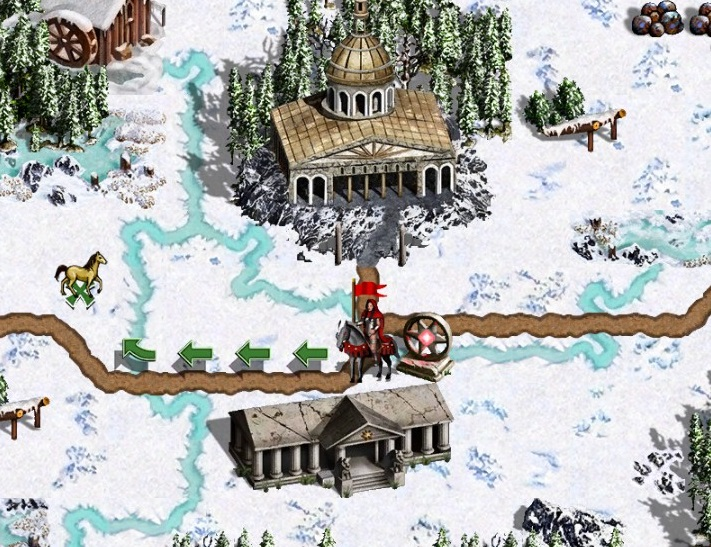
\includegraphics[width=0.85\textwidth]{heroes1.jpg}
\caption{Heroes 3 \label{heroes}}
\end{figure}
Algorytmy grafowe znajdują również zastosowanie w robotyce. Tego przykładem są roboty poruszające się w labiryncie, które muszą stworzyć jego mapę, będącą grafem, a następnie wyznaczyć najoptymalniejszą drogę do zadanego miejsca.

\section{Źródła}
\begin{itemize}
\item Thomas H. Cormen, Charles E. Leiserson, Ronald L. Rivest, Clifford Stein \textit{Wprowadzenie do algorytmów} wyd. VI
\item MIT OpenCourseWare (OCW) - wykłady profesora Patricka Winstona, dostępne na platformie \textit{YouTube}
\item Ubisoft Entertainment \textit{Heroes of Might and Magic III}
\end{itemize}


\end{document}